% --------------------------------------------------------------
% This is all preamble stuff that you don't have to worry about.
% Head down to where it says "Start here"
% --------------------------------------------------------------

\documentclass[12pt]{article}

\usepackage[margin=1in]{geometry}
\usepackage{amsmath,amsthm,amssymb}
\usepackage{tikz}

\newcommand{\N}{\mathbb{N}}
\newcommand{\Z}{\mathbb{Z}}

\newenvironment{theorem}[2][Theorem]{\begin{trivlist}
\item[\hskip \labelsep {\bfseries #1}\hskip \labelsep {\bfseries #2.}]}{\end{trivlist}}
\newenvironment{lemma}[2][Lemma]{\begin{trivlist}
\item[\hskip \labelsep {\bfseries #1}\hskip \labelsep {\bfseries #2.}]}{\end{trivlist}}
\newenvironment{exercise}[2][Exercise]{\begin{trivlist}
\item[\hskip \labelsep {\bfseries #1}\hskip \labelsep {\bfseries #2.}]}{\end{trivlist}}
\newenvironment{question}[2][Question]{\begin{trivlist}
\item[\hskip \labelsep {\bfseries #1}\hskip \labelsep {\bfseries #2.}]}{\end{trivlist}}
\newenvironment{proposition}[2][Proposition]{\begin{trivlist}
\item[\hskip \labelsep {\bfseries #1}\hskip \labelsep {\bfseries #2.}]}{\end{trivlist}}
\newenvironment{corollary}[2][Corollary]{\begin{trivlist}
\item[\hskip \labelsep {\bfseries #1}\hskip \labelsep {\bfseries #2.}]}{\end{trivlist}}

\begin{document}

% --------------------------------------------------------------
%                         Start here
% --------------------------------------------------------------

%\renewcommand{\qedsymbol}{\filledbox}

\title{Homework 3}%replace X with the appropriate number
\author{Dustin Lambright - dalambri \\ Aseem Raina - araina \\ Bihan Zhang - bzhang28 \\ Anshul Fadnavis - asfadnav\\
%replace with your name
CSC 565 - Graph Theory} %if necessary, replace with your course title

\maketitle


\begin{question}{1}
Show that every simple graph $G$ with 6 vertices has either a clique of size 3 or an independent
set of size 3.
\end{question}

Let $G$ be a graph of 6 vertices in the set $v$, named $a, b, c, d, e$, and $f$ \\ 

\textbf{i} $\deg(a) \geq 3$. Let us assume that $a$ is adjacent to $b, c,$ and $d$. If any of $b, c,$ or $d$ are adjacent to each other, they would form a clique of size 3 with $a$. If $b, c,$ or $d$ are non-adjacent they would form an independent set of size 3.\\

\textbf{ii} $\deg(a) < 3$. Let us assume that $a$ is not adjacent to any of $b, c,$ or $d$. If there are 2 independent sets in $b, c, d$ that would form an independent set of size 3 with $a$. The only way for $b,c,d$ to not have 2 independent sets among them would be for them to all be adjacent to each other, but they would then form a clique of size 3.\\

Thus $G$ either has a clique of 3, or an independent set of 3.  \\

Additionally, according to Ramsey's Theorem, the value of $R(3,3)$ is ${(3+3-2) \choose (3-1)}$, or ${4 \choose 2} = 6$, meaning a graph with a guaranteed independent set of size 3 or a clique of size 3 must have a $V(G) \geq 6$ \\


\begin{question}{2}
Prove or disprove: In a simple graph, every closed even trail of length more than 3 contains an even cycle.
\end{question}

To disprove the given statement, a single counterexample should suffice.\\
In the following simple graph, the closed even trail A-B-C-E-D-C-A of length 6:\\
\begin{align*}
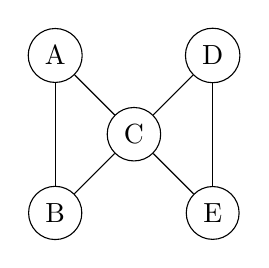
\begin{tikzpicture}
\node[shape=circle,draw=black] (B) at (1,0) {A};
\node[shape=circle,draw=black] (D) at (1,-2) {B};
\node[shape=circle,draw=black] (E) at (2,-1) {C};
\node[shape=circle,draw=black] (F) at (3,0) {D};
\node[shape=circle,draw=black] (H) at (3,-2) {E};
\path [] (B) edge node[left] {} (E);
\path [] (D) edge node[left] {} (E);
\path [] (E) edge node[left] {} (F);
\path [] (H) edge node[left] {} (E);
\path [] (B) edge node[left] {} (D);
\path [] (F) edge node[left] {} (H);
\end{tikzpicture}
\end{align*}
contains no even cycle. \\

\begin{question}{3}
Prove the following by strong induction on the length of the trail: The edge set of every closed trail can be partitioned into one or more pairwise edge-disjoint cycles.
\end{question}

Proof: Let $G$ be the graph containing the edge set $E$. \\

Let $n$ be the length of the maximum closed trial in $G$ of the form ($v_1$, $v_2$), ... ($v_n$, $v_1$). \\

Let $C$ be the smallest cycle in $G$ of the form ($v_i$, $v_{i+1}$)...($v_{i+k-1}$, $v_{i+k}$), where $v_i = v_{i+k}$ and $v_i$...$v_{i+k-1}$ are distinct (if the vertexes were not distinct that would mean it would be able to be partitioned into smaller cycles, and we started this exercise assuming C is the smallest cycle). \\

If $C = G$, the graph can be partitioned into one pairwise edge-disjoint cycle.\\

Otherwise, Let $G' = G - C$\\

The length of the closed trial through $G'$ cannot be more than $n$, and would have the closed trial ($v_1$, $v_2$)...($v_n$, $v_1$). \\

By induction we can partition the edge set of $G'$ into smaller disjoint cycles. Thus we show that the edge set of $G$ can be partitioned into disjoint cycles consisting of all the cycles in $G'$ and $C$\\


\begin{question}{4}
Suppose that $T$ is a maximal trail in a simple graph $G$ and that $T$ has at least one edge and is not closed. Prove that the endpoints of T have odd degree.
\end{question}

Let $v_1$ and $v_n$ be the endpoints of $T$ ($T$ must have at least 2 distinct vertexes, since it has at least one edge, and is not closed). \\

Since $T$ is not closed, $v_1$ and $v_n$ cannot be connected. \\

If $v_1$ had a neighbor $v_0$, and their connected edge was not in $T$, it must be added in $T$ in order for $T$ to be maximal. Thus $v_1$ can only have one neighbor, $v_2$. And any vertex, on a simple graph, with one neighbor has a degree of 1. The same argument can be applied to $v_n$ showing that it, also, has only one neighbor ($v_{n-1}$) and thus also has a degree of 1. \\

\begin{question}{5}
If $G$ is a graph with vertices $v_1, v_2, . . . , v_n$ and $A^k$ denotes the kth power of the adjacency matrix
of $G$ under matrix multiplication then \\ \\

(***) $A^{k}[i, j]$ is the number of $v_i, v_j$ -walks of length $k$ in $G$. \\ \\

Show how to use (***) to solve the following without multiplying matrices and prove your answer
correct: Let A be the adjacency matrix of $K_n$. If $i = j$, then $A^3[i, j]$ =\_\_\_\_ . Otherwise
$A^{3}[i, j]$ = \_\_\_\_.
\end{question}

Consider the graph $K_3$ ($n$ = 3).\\
Note: Although we've used $K_3$ to explain the derivation, this can be applied for any $K_n$.
\begin{align*}
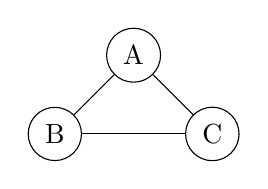
\begin{tikzpicture}
\node[shape=circle,draw=black] (A) at (1,1) {A};
\node[shape=circle,draw=black] (B) at (0,0) {B};
\node[shape=circle,draw=black] (C) at (2,0) {C};
\path [] (A) edge node[left] {} (B);
\path [] (A) edge node[left] {} (C);
\path [] (B) edge node[left] {} (C);
\end{tikzpicture}
\end{align*}

The expressions for these two cases can be derived as follows: 
\begin{center}
\Large TO CALCULATE (***) FOR $i \neq j$
\end{center}
\normalsize

There are 3 possible paths from A to C. \\
\begin{center}
\begin{tabular}{|c|}  \hline
\{AC, CA, AC\} \\
\{AC, CB, BC\} \\
\{AB, BA, AC\} \\ \hline
\end{tabular}
\end{center}

To calculate the number of walks of length 3 from source A to destination C, we could segregate them based on the first move:
\begin{enumerate}
\item to destination node C
\item to any other node except destination node C
\end{enumerate}
\begin{center}
\begin{tabular}{|c|}  \hline
\{AC, CA, AC\} \\
\{AC, CB, BC\} \\ \hline
\{AB, BA, AC\} \\ \hline
\end{tabular}


\begin{tabular}{|c|c|c|}
\multicolumn{3}{c}{BEGINNING MOVE TO C (THE END POINT)}  \\ \hline
MOVE TO & OPTIONS & REASONING \\ \hline
C & 1 & You can only move to C, as per definition \\ \hline
A or B &$n-1$ & Any option but C works for this step \\ \hline
C & 1 & The walk's third step has to end on C \\ \hline
\end{tabular} \\


\begin{tabular}{|c|c|c|}
\multicolumn{3}{c}{BEGINNING MOVE TO ANY OTHER POINT BUT THE END POINT}  \\ \hline
MOVE TO & OPTIONS & REASONING \\ \hline
B & $n-2$ & Any node except the current node A and destination node C \\ \hline
A or C & $n-2$ & C Any node except the current node B and destination node C \\ \hline
C & 1 & The walk's third step has to end on C \\ \hline
\end{tabular} \\
\end{center}

If we add these two options together, we get $(1 \times (n-1) \times 1) +  ((n-2) \times (n-2) \times 1)$, which simplifies to $n^{2} - 3n +3$ and can be re-written as $((n-1) \times (n-2)) + 1$. \\


The formula for calculating (***) $A^{3}[i, j]$ where $i \neq j$ therefore is $(n-1) \times (n-2) + 1$.

\begin{center}
\Large TO CALCULATE (***) FOR $i = j$
\end{center}
\normalsize

There are 2 possible paths from A to A. \\
\begin{center}
\begin{tabular}{|c|}  \hline
\{AB, BC, CA\} \\
\{AC, CB, BA\} \\ \hline
\end{tabular}
\end{center}

To calculate the number of paths, we have the following options: \\
\begin{center}
\begin{tabular}{|c|c|c|}
\multicolumn{3}{c}{STARTING AND ENDING AT THE SAME POINT}  \\ \hline
MOVE TO & OPTIONS & REASONING \\ \hline
B or C & $n-1$ & Any other node\\ \hline
C or B &$n-2$ & Any node except the current node and destination node A \\ \hline
A & 1 & The walk's third step has to end on A \\ \hline
\end{tabular} \\
\end{center}

When we combine these, we get $(n-1) \times (n-2) \times 1$.

The formula for calculating (***) $A^{3}[i, j]$ where $i = j$ therefore is $(n-1) \times (n-2)$.

For reference, $A^{3}[i,j]$ is:
\begin{tabular}{|c|c|c|c|} \hline
 & A & B & C \\ \hline
 A & 2 & 3 & 3 \\ \hline
 B & 3 & 2 & 3 \\ \hline
 C & 3 & 3 & 2 \\ \hline
 \end{tabular} \\ \\
 This is the result of cubing $K_3$, and applying the formula above. \\

\begin{center}
\Large IN CONCLUSION \\

\normalsize
$ A^{3}[i,j] = $ 
    $\begin{cases} (n-1) \times (n-2) + 1  & \mbox{if } i \neq  j  \\  (n-1) \times (n-2)   & \mbox{if } i =j \\   \end{cases}$ \\
    where $n$ is the number of vertices in $G$. \\
\end{center}

\begin{question}{6}
Draw a simple, connected graph with the following degree sequence, or prove that no such graph
is possible: \\
a. (3, 3, 3, 2, 2, 2) \\
For any graph G, the number of vertices of odd degree should be even. Here, we have 3 vertices of odd degree (3,3,3), hence no such graph is possible. \\
b. (7, 6, 5, 4, 3, 2, 1) \\
No such graph is possible as a vertex cannot have degree equal to the total number of vertices in a simple graph (i.e. 7). \\ \\
c. (3, 3, 2, 2, 1, 1) \\
A graph is possible \\
\begin{align*}
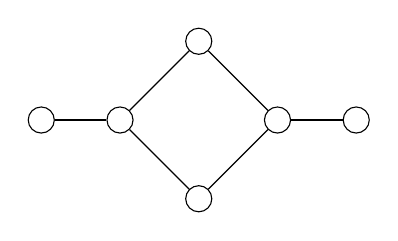
\begin{tikzpicture}
\node[shape=circle,draw=black] (A) at (-1,0) {};
\node[shape=circle,draw=black] (B) at (0,1) {};
\node[shape=circle,draw=black] (C) at (1,0) {};
\node[shape=circle,draw=black] (D) at (0,-1) {};
\node[shape=circle,draw=black] (E) at (-2,0) {};
\node[shape=circle,draw=black] (F) at (2,0) {};
\path [] (A) edge node[left] {} (B);
\path [] (B) edge node[left] {} (C);
\path [] (C) edge node[left] {} (D);
\path [] (D) edge node[left] {} (A);
\path [] (A) edge node[left] {} (E);
\path [] (C) edge node[left] {} (F);
\end{tikzpicture}
\end{align*}
d. (7, 6, 5, 4, 3, 3, 2) \\
No such graph is possible as a vertex cannot have degree equal to the total number of vertices in a simple graph (i.e. 7). \\
e. (6, 6, 5, 4, 3, 3, 1)\\
For the given sequence of seven vertices, two vertices have degree 6. For such a simple graph to exist, all vertices must have a degree of at least 2. Since one vertex has degree 1, such a graph is not possible.
\end{question}

\begin{question}{7}
 How many different simple graphs are there with 5 edges and with vertex set {v1, v2, . . . v5}?
(We are counting labeled graphs, not isomorphism classes)
\end{question}

Consider the following adjacency table for 5 vertices. There are $(5-1)!$ places to place an edge, so the number of different simple graphs is ${10 \choose 5}= 252$


	\begin{tabular}{c|c|c|c|c|c|}
		\cline{2-6}
		& v1 & v2 & v3 & v4 & v5 \\
		\hline
		\multicolumn{1}{|c|}{v1} & 0 & - & - & - & - \\
		\hline
		\multicolumn{1}{|c|}{v2} &   & 0 & - & - & - \\
		\hline
		\multicolumn{1}{|c|}{v3} &   &   & 0 & - & - \\
		\hline
		\multicolumn{1}{|c|}{v4} &   &   &   & 0 & - \\
		\hline
		\multicolumn{1}{|c|}{v5} &   &   &   &   & 0 \\
		\hline
	\end{tabular}


\begin{question}{8}
Prove by contradiction: A graph with every vertex degree even has no cut-edge.
\end{question}

Let us assume that there does exist a cut-edge $e$ in graph $G$ (where every vertex has an even degree), joining vertices $v_i$ and $v_j$.\\
Removing $e$ would divide $G$ into two the following two graphs:\\
$G_1$: containing $v_i$ (now with an odd degree, since $e$ was removed) and zero or more vertices with an even vertex degree.\\
$G_2$: containing $v_j$ (now with an odd degree, since $e$ was removed) and zero or more vertices with an even vertex degree.\\
Since no graph can have an odd number of odd-degree vertices, neither $G_1$ nor $G_2$ can exist.\\
This means that our assumption was false.\\
Hence we have proven that a graph with every vertex degree even has no cut-edge.




% --------------------------------------------------------------
%     You don't have to mess with anything below this line.
% --------------------------------------------------------------

\end{document}
